\chapter{Code Rationales for \break Neural Language Models}
\label{ch8:rationales}

%Approach
Although multiple deep learning studies work on code generation by means of language modeling \cite{Cruz-Benito}, literature shows that those studies focus mainly on traditional machine learning metrics  (i.e., loss and accuracy metrics to evaluate the results obtained by the generative process) omitting interpretability methods. Thus, the development of tailored methods for interpretability of \textit{Code Generation} remains unexplored. Unfortunately, interpretability methods have been omitted in recent studies of deep learning for software engineering. This patent lays out a formalization to introduce an interpretability method, called \codeSeqRational, that can assist researchers to understand neural code generation. The goal of this patent is to design and develop an automated, effective, and practical interpretability approach for identifying underlying features of code generators. 

Our approach \codeSeqRational is based on a proposed greedy algorithm know as \textit{sequence rationales}\citep{vafa2021rationales}, which finds the minimum set of words that most contribute for the prediction of a specific token. Such set of words can be employed to generate local or global explanations of a NLM. Local post-hoc interpretability aims at generating an explanation for a single sample, while global post-hoc interpretability generates explanations for a whole model. 

Firstly, \textit{Sequence rationales} adapted to source code provide a fine-grained (token-level) and local (single sample) interpretation of generated output. Secondly, on top of this, our approach defines a set of mapping functions which assign each token to a hierarchy of code and natural language concepts. In practice, a semantic parser is used to analyze the input and output of the model. The parser is able to identify code and natural language tokens, recognize tokens and assign them to different categories based on the token's role. For example, the token \texttt{foo} in the statement \texttt{int foo = 5;} is recognized as a variable name (low-level category), which is part of the identifiers (higher-level category). Thirdly, the token is assigned to a scope category based on its location within the input code (\eg package, class, or method level). Lastly, once these tokens are classified in different levels and categories, \codeSeqRational offers several functions to aggregate rationales from the tokens of each category. For example, the variable name category (\ie all tokens representing variable names) and method name category can be compared in terms of how much they contribute to the output generation, for the given code task at hand.

Furthermore, \codeSeqRational offers a methodology and infrastructure to obtain interpretability insights about NLM on code. This framework enables researchers, AI practitioners, and customers to produce explanation which can be useful in several practical scenarios. Specifically, our infrastructure can be used two-fold for \textit{debugging} and \textit{optimizing} NLMs for code generation and code-related tasks. 

Although interpretability is a young field in ML, producing explanations can be very useful for debugging generative models. On the one hand, interpretability insights provided by \codeSeqRational can be used to investigate specific output generation, for example an incorrect variable token in the generated code snippet. Additionally, global explanation could be extracted for classes/set of output (\eg syntactically incorrect generation, failing tests, code containing security issues), guiding the researchers and practitioners towards the resolution. On the other hand, the optimization would focus on finding parts of the training data (or sets of tokens) that most contribute to code generation. Our method \codeSeqRational can be used to optimize the input space for different code-related tasks, based on the type of tokens (\ie natural language or code), categories (\ie identifiers, code structure), and scopes (\ie package, class, methods) which most influence the generation for particular tasks. For example, a source code file could be used as input to different code task, such as completing the current method, generating documentation, or test cases. However, these tasks could focus on different types of tokens and scopes, thus optimizing the input for each task could lead to performance improvements, for example by removing unnecessary parts of the input (noise) and allowing more informative tokens. This is particularly important given the limited-size of the input to NLM (often limited to 1024 tokens).

%------------------------------------------------

\section{Background Formalization}

\subsection{Neural Language Models for Code}

One common barrier to the practical adoption of any \textit{ML} model is that such models often omit explanations for their output~\citep{molnar2019interpret}. These explanations must be presented in understandable terms to a human in order to facilitate confidence for model deployment~\citep{Doshi-Velez2018ConsiderationsLearning}. In this context, \textit{Interpretable Machine Learning} refers to methods and models that make the behavior and predictions of ML systems understandable to humans.  Our proposed \codeSeqRational evaluation method aims at enabling Interpretable NLMs for code. The usage of Deep Learning Models and, specifically, Neural Language Models (NLM) in Software Engineering has seen striking advances with regard to code generation and downstream SE tasks \citep{Chen2021EvaluatingCode, watson2020dl4se}. Nonetheless, researchers are unable to establish what aspects of code are actually learned by modern neural models. In this section, we present the necessary background regarding NLMs. 

Neural Language Models (NLM) have been employed in Software Engineering as a technique to approximate \textit{Code Generators} $\mathcal{G}_c$. There are other definitions for these models according to their size and architecture. We can find the concept of \textit{Large Language Models (LLM)} \citep{Bender2021OnBig} or, more recently, \textit{Foundation Models} \citep{Bommasani2021OnModels}. Regardless the model name, all of them are modeling or representing sequences using deep neural networks. 

In the context of SE, the goal of a language model is to find a representation of a software artifact. Software artifacts can be represented as sequence-based data consisting of tokens (\eg source code, requirements, or test cases). While other representations exist, such as graph-based models~\citep{allamanis2018learning}, we focus our discussion on sequence-based models for simplicity. We refer to SE-specific sequence-based data as software corpora $\mathcal{C}$. Given the sequential nature of $\mathcal{C}$, we can decompose $\mathcal{C} = w_1,...,w_T$ into a desired granularity of tokens, words, or sub-words \citep{Karampatsis2019} by using a transformation function $\Gamma(\mathcal{C})$. This transformation function is a tokenization method for converting a software corpus into a sequence of discrete objects $w_t$  for $1 \leqslant t \leqslant T$. Note that $w_t \in V$, where the vocabulary $V$ is a finite set. 

Given this definition, a statistical language model is a probability distribution $P_{\theta}$ over a fixed granularity of sequences $\mathcal{S}$ of software corpora $\mathcal{C}$. We can factorize the joint distribution over the $t-$dimension as in \equaref{eq:llm}. 

\marginnote{
\begin{align}
\begin{split}
P_{\theta}(\mathcal{S}) & = P_{\theta}(w_1,...,w_T) \\
                        & = \prod_{t = 1}^{T} P_{\theta}(w_t | w_{t-1},...,w_1 )
\end{split}
\label{eq:llm}
\end{align}
}

Due to the discrete nature of the data, the expression $P_{\theta}(w_t | w_{t-1},...,w_1 )$ can be estimated using a classifier. The classifier, in our particular case, is a neural language model (NLM) \citep{Bengio2003AModel}. Hence, rather than using \textit{n}-grams or Markov Models to approximate $P_{\theta}(w_t | w_{t-1},...,w_1 )$ \citep{Karampatsis2020Open-VocabularyAbstract}, it is convenient to use a latent model $P_{\theta}(w_t | w_{t-1},...,w_1 ) \approx P(w_t | h_t )$, where $h_t$ is known as a \textit{hidden state} that embeds the sequence information from past observations up to the time step $t$.

Depending on \textit{how} the sequence is processed, the hidden state $h_t$ can be computed using either an autoregressive network (\ie such as a Transformer~\citep{vaswani2017transformers}) or recurrent neural network (RNN). Autoregressive models update the hidden state $h_t = f(h_{t-1}, w_{<t})$ using past inputs $w_{<t}$ and a previous hidden state $h_{t-1}$. Conversely, recurrent models update the hidden state $h_t = f(h_{t-1}, w_{t})$ using just the current input $w_{t}$ and a previous hidden state $h_{t-1}$. In other words, autoregressive models function in a feed-forward manner that predict future values from historical values directly, while recurrent models predict future values from past information encoded into a hidden state. 
Our proposed \codeSeqRational methodology is designed to be compatible with either type of NLM.

\textbf{Special Case: Encoder-Decoder Architecture.} For language models used in machine translation, sequences $\mathcal{S}$ can be decomposed into input $\mathcal{S}_v = v_{<M}$ and output $\mathcal{S}_w = v_{<T}$. Thus, \equaref{eq:llm} is updated to include an input sequence:

\begin{align}
\begin{split}
P_{\theta}(\mathcal{S}_v,\mathcal{S}_w) & = P_{\theta}(v_1,...,v_M,w_1,...,w_T) \\
                        & = \prod_{t = 1}^{T} P_{\theta}(w_t | w_{<t}, v_{1:M} )
\end{split}
\label{eq:llmML}
\end{align}

\textbf{Modeling Long Range Code Dependencies.} NLMs trained on source code have the ability to generate tokens or sub-words given a history. Hence, these models are employed as generative models $w_t  \backsim P(w_t | w_{t-1},...,w_1 )$. Both autoregressive and RNN models share a common property: \textit{the ability to connect previously processed information to a present task, such as using an initial sequence of tokens to predict new code tokens}. The resulting auto-completed sequence should be coherent in relation to the context of the initial sequence. That is, the predicted token $w_t$ is \textit{conditioned} by the previous information. This property is known as the ability to model \textit{long-range or long-term dependencies}~\citep{karpathy2015understand}.

\begin{equation}
\hat{w_t} = P_{\theta}(w_t | w_{t-1,...,w_1} ) = \sigma(y)_t = \frac{e^{y_{w_t}}}{\Sigma_i e^{y_i}}
\label{eq:long}
\end{equation}

\noindent In the above equation, $y_i$ represents the non-normalized log-probabilities for each output token $i$. This estimation relies on the softmax function. The softmax $\sigma_t$ returns a distribution over predicted output classes, in this case, the classes are each token in the previously introduced vocabulary $V$. 
It is expected that the predictions contained in $\sigma_t$ are influenced by previous inputs of the sequence 

\begin{equation}
H(P,Q) = - \sum_{t \in T} P(w_t | h_t) \log Q(w_t | w_{<t})
\label{eq:cross}
\end{equation}

In past SE studies on NLMs for code, models have typically been evaluated without explicitly investigating their ability to model long range dependencies. \equaref{eq:cross} is typically used to depict the cross-entropy loss, notice that the term $Q(w_t| W_{<t})$ represents the approximated distribution of the ground truth using a one-hot vector.

%------------------------------------------------

\section{Code Sequential Rationales}

We present and describe \codeSeqRational: an approach designed to provide an automated and effective way to extract practical interpretability insights for NLM-based systems for code-related tasks. The approach \codeSeqRational is composed of three stages: \underline{A) Code Rationales:} Given a Neural Language Models (NLM) trained on a code-related task (\ie code completion, program repair, translation, or test generation), we rely on a proposed greedy algorithm know as \textit{sequence rationales} or \textit{greedy rationalization} \citep{vafa2021rationales} to understand NLM generation. Greedy rationalization finds the the minimum set of words that most contribute for the prediction of a specific token. In particular, for each token predicted by the NLM, greedy rationalization assigns rationales (numerical values organized in sets) to all input tokens or context window. \underline{B) Local post-hoc rationales:} Using a set of rationales to explain a single sample can be less informative if we operate over tokens without considering other code properties. That is the reason why we use \textit{human-interpretable concepts} to provide further understanding of a set of rationales for a single sample. Such concepts are obtained by using mapping functions or parser machines. And \underline{C) Global post-hoc rationales:} Once the set of rationales is aggregated for a single sample, we can escalate local post-hoc rationales methodology for whole sample set. By executing greedy rationalization on a sample set, we can observe a global behaviour of the NLM. 


\subsection{Code Rationales}
Rationales are subsets of input tokens from the context window that can \textit{explain} individual model predictions. By using combinatorial optimization, we are able to find the smallest subset of tokens that predict the same output as the full set of tokens. Such smallest subset are considered the best rationale. Vafa, et all introduce a strategy to approximate the \textit{best rationale} since enumerating all possible subsets is intractable. This strategy uses a greedy algorithm: \textit{greedy rationalization}. In order to use this greedy algorithm in any model, we must make the model "compatible" for a given combination of subsets of the input context. 

Consider the code sequence  $\mathcal{S} = w_{1:T}$, where the token $w_t$ is predicted given the context window $w_{<t}$ at any token position $t$. A sequence model $P_{\theta}$ is a probabilistic model that approximates a code generator $\mathcal{G}_c$ from samples $\mathcal{S}^n$, $n$ is the number of samples used for learning a model $p_{\theta}$. A code rational $r_w \subset w_{<t} $ is a subset of a context window $w_{<t}$ that can explain a prediction $w_t$.

The power set $\mathcal{R} = 2^{[t-1]}$ is the set of all possible subsets for the sequence context $w_{<t}$. The purpose of code rationales is to find a subset $r_w \in \mathcal{R}$ that achieves the same prediction as the context $w_{<t}$. Additionally, such rationales should be as smaller as possible $\hat{r_w}$ so that the interpretation of the token $w_t$ becomes as clearer as possible too. Take into consideration that predicting a token $w_t$ depends upon the context $w_{<t}$, while predicting a token $w'_t$ depends on the optimal rational $w_{r_w}$. Thus, code rationales are formulated as a combinatorial problem

\begin{equation}
r(w_{1:T}) = \arg \min_{r_w \in \mathcal{R}} |r| : \arg \max_{w'_t} P_{\theta}(w'_t|w_{r_w}) = w_t
\label{eq:combinatorial}
\end{equation}


Vafa et al., highlighted two main computational problems to solve objective function \equaref{eq:combinatorial}: 1) the optimization problem is intractable or NP-hard, and 2) evaluating conditioned distributions on subsets $w_r$ is also intractable over missing tokens. The first problem is solved by means of \textit{greedy rationalizations}, an algorithm to approximate a solution for \equaref{eq:combinatorial}. The second problem is solved using model \textit{compatibility}.

\textbf{Greedy rationalization} algorithm starts with the empty set adding iteratively the rationale that most contributes to the probability of $w_t$ at each step. Since the power set starts with the empty set 
$$r^{(0)}=\emptyset$$
the first rationale set is defined as
$$r^{(1)} = \arg \max_{j \in \{ [t-1] \} } P_{\theta}(w_t|w_j)$$
we can keep adding tokens to configure the rationale by choosing the sequence that maximizes the probability of the token $w_t$ at each step

\begin{equation}
r^{(k+1)} = r^{(k)} \cup  \arg \max_{j \in \{[t-1] \setminus r^{(k)} \} } P_{\theta}(w_t|w_{ \{ r^{(k)}\cup j \} })
\label{eq:greedy}
\end{equation}

The halting condition for the previous expression is, precisely, the \equaref{eq:combinatorial} when $ \arg \max_{w'_t} P_{\theta}(w'_t|w_{r^{(k)}}) = w_t$.  Note that a rational is the set of tokens that \textbf{covers} a given sequence $\mathcal{S}$ if such rational predicts a target token $w_t$. The algorithm described in Eq~\ref{eq:greedy} always converge because the edge case $r^{(k-1)}$, which is the worst case, is guarantee to contain the entire context window $w_{<t}$. 

For conditioned models employed in \textit{machine translation}, an input sequence $v_{1:M}$ generates an output sequence $w_{1:T}$. In this particular model, the predicted token $w_t$ depends on both input $v_{1:M}$ and output $w_{<t}$. Therefore, the candidate rationales is defined as the cross product of power sets $\mathcal{R} = 2^{[M]}\times 2^{[t-1]}$. The combinatorial \equaref{eq:combinatorial} is updated to include the input sequence:

\begin{align}
\begin{split}
r(v_{1:M},w_{1:T})  & = \\
\arg \min_{r_v,r_w, \in \mathcal{R}} |r_v| + |r_w| : \arg \max_{w'_t} P_{\theta}(w'_t|v_{r_v},w_{r_w}) \\
                    & = w_t
\end{split}
\label{eq:combinatorialMT}
\end{align}

\textbf{Model compatibility} is a property for approximating the distribution $P_{\theta}(w_t|w_r)$ using $F_{\theta}(w_t|w_r)$. The function $F_{\theta}$ in \equaref{eq:llm2} is a concrete model (e.g., Transformer, Recurrent Nets, or n-grams) trained on complete subsets $w_{<t}$. Alas, such model were not trained on incomplete context $w_r$. We need those incomplete context or subsets of $w_{<t}$ to enable \textit{greedy rationalizations}.

\begin{align}
\begin{split}
P_{\theta}(\mathcal{S}) & = P_{\theta}(w_{1:T}) \\
                        & = F_{\theta}(w_1)\prod_{t = 2}^{T} F_{\theta}(w_t | w_{<t} )
\end{split}
\label{eq:llm2}
\end{align}

Therefore, compatibility can be achieved by fine-tuning on incomplete context $w_r$. Since $F_{\theta}$ is already trained on complete context, the compatibility process will not affect the performance of original downstream tasks. 

\begin{figure}[t]
\caption{Human-interpretable Concepts $\mathcal{H}$ }
\centering
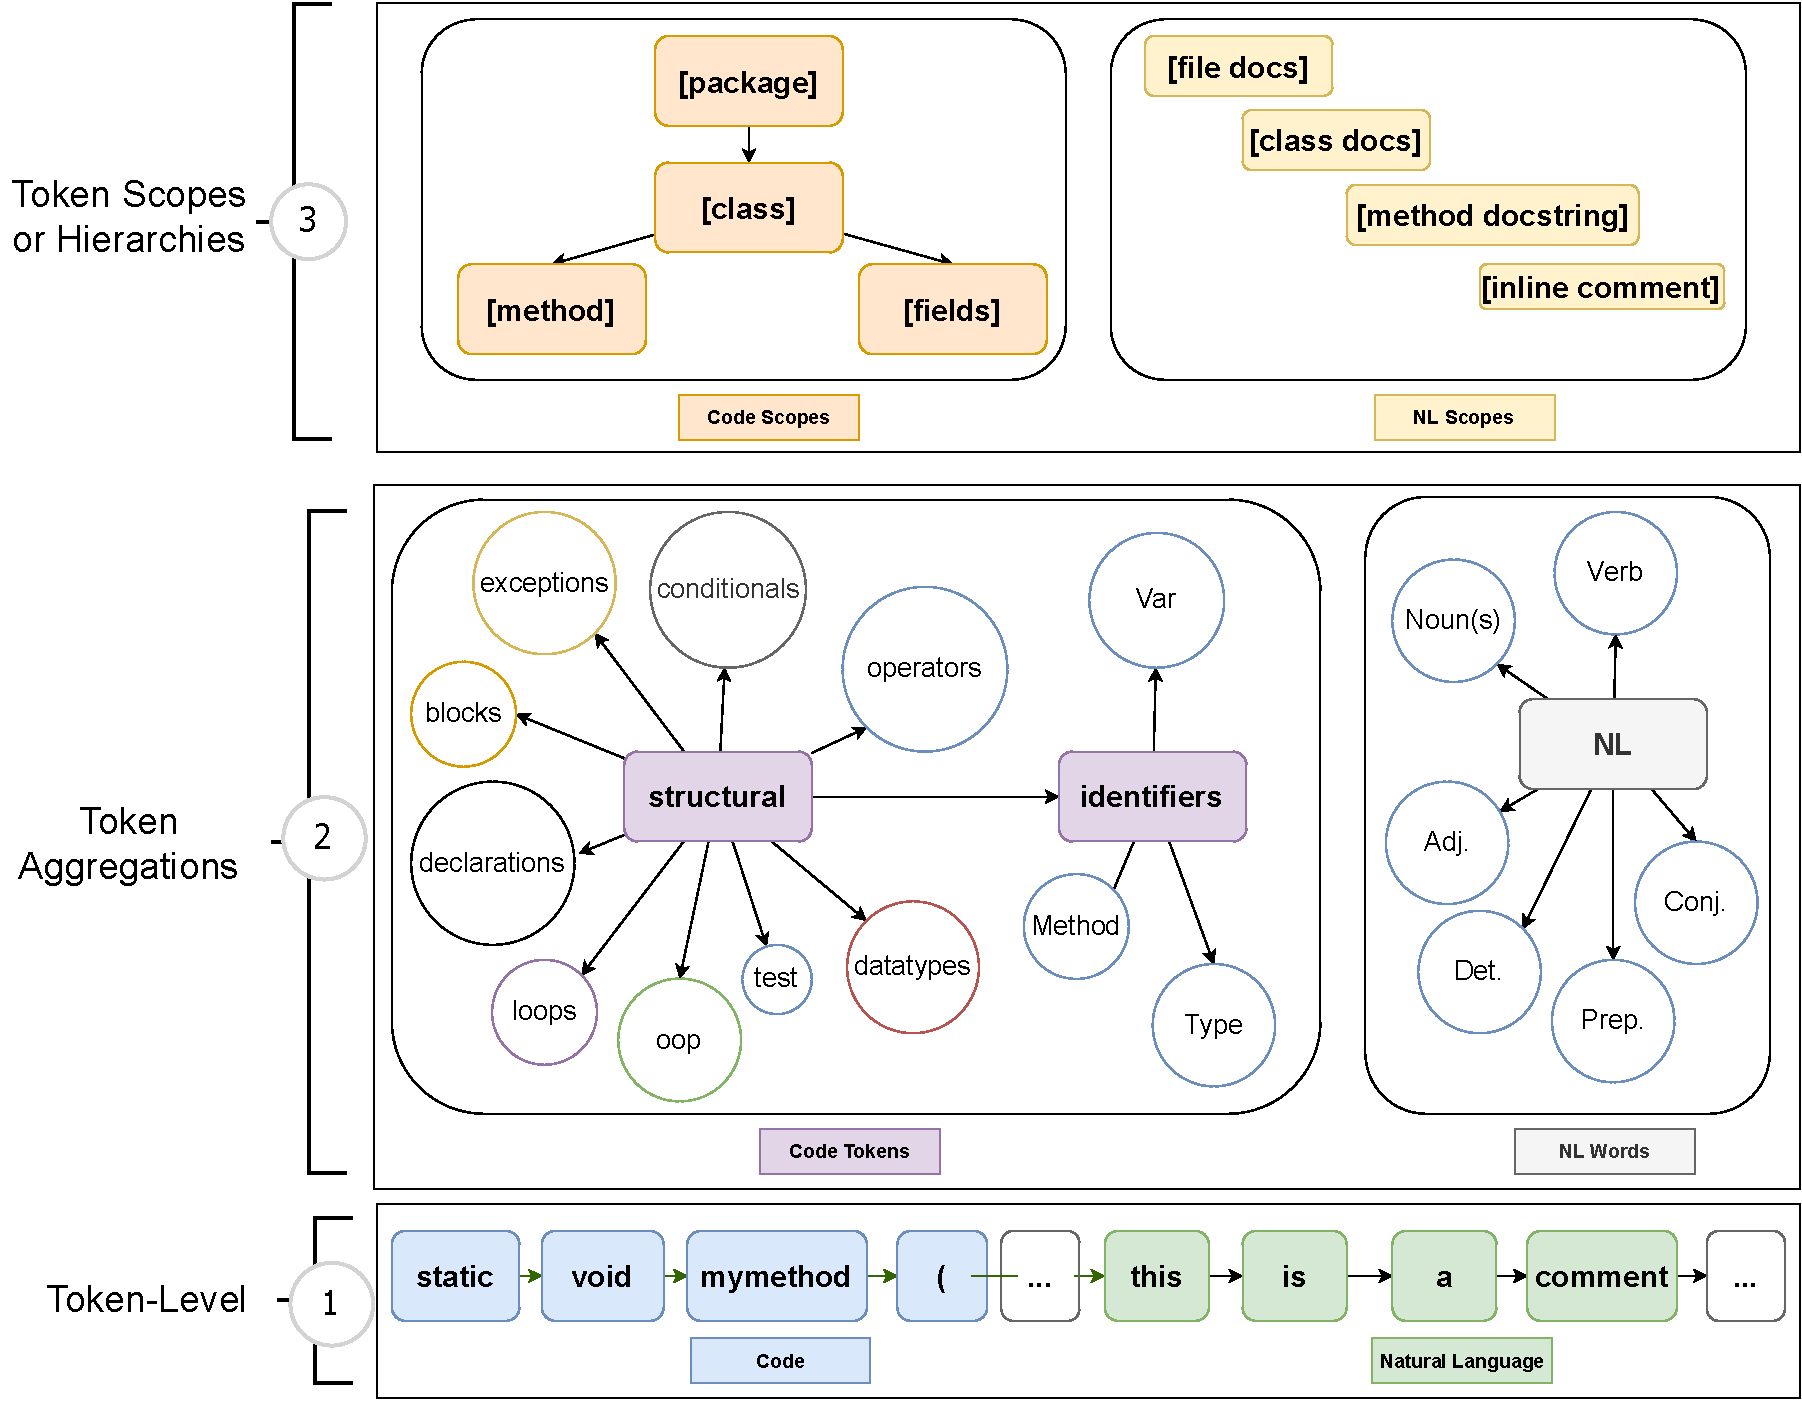
\includegraphics[width=0.9\textwidth]{graphics/chap_08-interpret-rational/fig_1_humanConcepts.pdf}
\label{fig:human}
\end{figure}


\textbf{Complexity Analysis.} In particular, Vafa et al. offer a complexity analysis for the \textit{greedy rationalization} algorithm. The analysis can be segmented in three parts: I) searching the min set of rationales in $m$ steps is $O(m)$; II) searching the max probability of $w'_t$ across $t$ is $O(t)$; and III) computing $F_{\theta}(w_t|w_{<t})$ is quadratic $O(t^2)$, in particular, for transformers. Note that in each step of the greedy rationalization, the term $F_{\theta}(w'_t|w_{r_w})$ must be evaluated, which means a complexity of $O(m^2)$ for a rationale size $m = |r|$. Therefore, if it is assumed that $m < t$, then the greedy rationalization is completed altogether in $O(m^3t)$ steps. Bear in mind that evaluating a transformer for an input $t$ would require $O(t^2)$; greedy rationalization has the same asymptotic complexity as evaluating a transformer if the rationale size $m=t^{1/3}$.

\subsection{Local post-hoc code rationales}

Most NLMs operate upon features, such as a token prediction $P(w_t|h_t)$, that do not \textit{inherently} match high-level concepts a human can easily understand. Such difficulty can be expressed mathematically as representing the state of a machine learning (ML) model as a vector space $\Vec{l}$, which corresponds to data as input features $\mathcal{S} = w_{1:T}$. Conversely, developers operate in a different vector space $\Vec{h}$, which corresponds to a set of human-interpretable concepts $\mathcal{H}$. Interpreting an $P_{\theta}$ model can be formalized as:

\begin{equation}
\phi: \Vec{l} \to \Vec{h}
\label{eq:kim}
\end{equation}

The function $\phi$ is known as \textit{function for interpretability} \citep{Kim2018InterpretabilityTCAV}. This function could adopt many forms (e.g., linear, quadratic, or polynomial) and, therefore, it may not capture all the aspects of its input domain, $\Vec{l} \in \mathcal{S}$, and it may not cover all possible human concepts in $\Vec{h} \in \mathcal{H}$. 

Post-hoc explanations occur after training a code generator $\mathcal{G}_c$. A local post-hoc explanation is the result of the interpretability function $\phi(\mathcal{S},\mathcal{H})$ for a single code sequence $\mathcal{S}$ in terms of \textbf{Human-interpretable concept} $\mathcal{H}$. \equaref{fig:human} shows three levels of human-interpretable concepts: 1) token-level, 2) token aggregations, and 3) token scopes (or hierarchies). In fact, the function \equaref{eq:kim} can be virtually \textit{code rationales} with the form $\phi_0(w_{1:T}, \mathcal{H}^{(0)}) = r(w_{1:T})$ if we consider a rationale a \textit{human-interpretable concept} $\mathcal{H}^{(0)}$. Then, $\phi_0$ would be pure analyses of rationales at token-level. 

However, we could define an extra layer of interpretability beyond reporting tokens within a rationale as depicted in \equaref{fig:human}. Such tokens can be organized or semantically grouped by their function. \equaref{fig:human}-2 presents two-fold aggregation functions depending upon the nature of tokens: code or natural language. Particularly, we proposed a \textit{structural code taxonomy for java} as a first attempt to locally aggregate code rationales $r(\mathcal{S})$ by structural categories (see \equaref{fig:taxonomy}). These categories $\mathcal{H}^{(1)}$ are high-level properties of code that can be mapped from token-level rationales. Using this taxonomy, we are able to interpret NLM predictions in a developer-centric way. In programming languages (PL), different types of tokens retain different semantic meanings. For instance $=$ and $<$ are common \textit{operators}. As such, we can group tokens into semantically meaningful categories that we call \textit{structural concepts} (see \equaref{fig:human}-2). These features will allow us to assign semantic meaning to results when analyzing rationales $r$ by defining 

\begin{align}
\begin{split}
\phi_1(\mathcal{S}, [\mathcal{H}^{(0)},  \mathcal{H}^{(1)}])  & = \lambda_{\mathcal{H}^{(1)} } ( \phi_0(\mathcal{S}, \mathcal{H}^{(0)} ) \\
                                                            & = \lambda_{\mathcal{H}^{(1)} } ( r(\mathcal{S}) )
\end{split}
\label{eq:structuralagg}
\end{align}

The mapping function $\lambda_{\mathcal{H}^{(1)}}$ receives a set of rationales of a concrete sequence $\mathcal{S}$ to generate a local explanation in terms of the structural code taxonomy. This explanation is obtained by aggregating rationales by the categories defined in the taxonomy throughout descriptive statistical function (e.g., mean, median, max, etc). Note that new taxonomies for different PLs can be derived/used. The mapping function $\lambda_{\mathcal{H}^{(1)}}$ is, indeed, a parser. This parser could translate or identify categories for a given token (e.g., operators, blocks, or loops) or word (e.g., verb, noun, or adjective). 

We can even go a little bit further and define code concepts by extracting and grouping topics from identifiers (natural language) (see \equaref{fig:human}-2). We refer to these taxonomy as \textbf{Identifier Concepts} $\mathcal{H}^{(2)}$. Here, the mapping function $\lambda_{\mathcal{H}^{(2)}}$ can be defined as an unsupervised approach to generate clusters from semantic embedded in variable names and comments. 



\textbf{Code Context Scopes} $\mathcal{H}^{(3)}$ are other type of suggested taxonomy (see \equaref{fig:human}-3). Oftentimes, it is difficult to predict whether a given NLM will be used in a similar setting to its corresponding sanitized training or testing set. For instance, if a model trained on a well-commented dataset is applied to predict segments of poorly commented code, this could potentially impact performance. As such, we define \textit{Code Context Scopes} to better understand model performance across different hierarchies or levels of context windows.  We formulate these interpretable settings as testbeds (\ie datasets) organized in context scopes. For instance, a testbed oriented to "method scope", may consist of testbeds with such level. Therefore, these datasets describe the Long Range Code Dependency property, which we introduced in the background section. Currently, \codeSeqRational supports both code and natural language scopes. For code scopes $\lambda_{\mathcal{H}^{(3)}}$, four elements are identified: (i) package, (ii) class, (iii) method, and (iv) fields (see \equaref{fig:human}-3). We can also extent the scopes to include signatures or higher level components. We support also custom mapping functions could aggregate tokens at different scopes, highlighting specific parts of the input that are particularly interesting for the downstream task at hand. For example, tokens belonging to a specific method could be aggregated in a specific category (different to other methods), if that method within has a particular role in the taks (\eg a \textit{focal} method for test generation task, a \textit{buggy} method in program repair task).

Following the same logic, other type of categories can be defined in terms of scopes without necessarily implying code hierarchies. We also introduce \textbf{Natural Language-Based Scopes} $\mathcal{H}^{(4)}$ that aggregate code rationales by file docs, class docs, method docstring, and inline comments (see \equaref{fig:human}-3). We may use a distinct mapping function $\lambda_{\mathcal{H}^{(4)}}$ based on code parser as well. 

\subsection{Global post-hoc code rationales}

Global explanations $\Phi(g,\mathcal{S}^n)$ are relevant to understand the overall behavior of a neural language model $\mathcal{G}_c$. We must define an aggregation function $g(\phi,\mathcal{S}^n)$ and a sample $n$ of sequences $\mathcal{S}^n$. Aggregation functions might vary depending on the desired statistical treatment. Even thought, global methods should always describe how input features impact model predictions on average. We suggest, in fact, employing expected values:

\begin{equation}
\Phi(g,\mathcal{S}^n,\mathcal{H}) =  g(\phi_{\mathcal{H}},\mathcal{S}^n) = \frac{1}{n} \sum_{j=1}^{n} \phi_{\mathcal{H}}(\mathcal{S}^j,\mathcal{H})
\label{eq:aggregation}
\end{equation}

Note that global explanations can be tuned for a specific \textit{human-interpretable concept} $\mathcal{H}$. We can observe how, for example, \textit{structural code} categories affect the overall prediction behavior for a given model $\mathcal{G}$. 

%------------------------------------------------

\section{Applications}
\label{sec:applications-rationales}

Although \textit{interpretability} is about \textit{why} a prediction or model decision was made, our approach supports two main applications for interpretability of NLM for code-related tasks: \textit{debugging} and \textit{optimization}. These applications can be used by researchers and practitioners designing NLM-based solutions.

\subsection{Debugging}
Debugging concerns the investigation process aiming at understanding and resolving a specific problem (or bug). In this context, debugging an NLM trained on code generation task is challenging. Differently from traditional solutions based on declarative code and rules which could be investigated and modified in order to resolve a bug, an NLM-based approach has million of parameters that contribute to the generation of an output. Our approach, provides interpretability insights to link errors to specific parts of the input to the model.

%Detecting bias

\textbf{Local Scenario,} An NLM for code completion generates a personal identifiable information within a code statement. The ML engineer of the model uses \codeSeqRational to link the generated token (personal information) to the input tokens that contributed the most to this generation. The ML engineer inspects these tokens and defines rules to abstract such tokens in the training set, so that the newly trained model will avoid similar generations in the future. 


\textbf{Global Scenario.} A code generation model makes two categories of mistakes, classified as $A$ and $B$. The ML engineer of the model collects different samples for the categories  $A$ and $B$, and uses \codeSeqRational to extract rationales, aggregate them over the two sets, and extract interpretability insights from them at code context scope level. The ML engineer discovers that the errors are originated from two scopes (\eg package and class). This information is used to change the input of the model.


\subsection{Optimization}
NLM take as input a limited-size sequence of tokens, often capped at 1024 tokens, from which the model generates an output. Given the limited nature of the input size, it is fundamental that the input space is used effectively, providing the model with the important information (tokens) while minimizing noise. Recent papers have shown the importance of providing contextual information to NLM for code generation \cite{clement2021long}, but the limited-size input of the models requires engineers to carefully decide what information to incorporate in the input. Our approach can guide ML engineers on deciding which parts of the input constitute important information to include for a specific code task.

\textbf{Global Scenario.} Two NLMs have been trained for two code-related tasks $A$ and $B$. These models both take as input a source code file. However, since some source code files are quite large, the input is often truncated. The ML engineer wants to understand what parts of the input are more important for task $A$ and $B$, so that it can optimize the input for each task. Our approach is used to generate rationales and grouped them at different code scopes. The results indicate that method docstrings are particularly important for task $A$, while class information are more influential for task $B$. This information is used by the ML engineer to optimize the input for each task. 

\subsection{Insights}
Our approach can be used to validate hypotheses on feature/token importance for specific code tasks and guide model improvements. Researchers and practitioners can use \codeSeqRational to extract interpretability values, aggregate them at different levels, and test hypotheses on the influence of class of tokens on the generated output. 